In Abbildung 2.5 ist ein Überblick zu sehen, welche Schritte nötig sind, um TPT für einen Test einzurichten \parencite[S. 39]{userguide}. 
%Im Folgenden ist zu sehen, welche Schritte benötigt werden, um TPT für einen Test einzurichten:
\begin{figure}[!h]
    \centering


  \begin{tikzpicture}%[every node/.style={rectangle,draw,text width=14em,align=center}]
    [
      % Stil für Ein- und Ausgabe
      io/.style={trapezium, trapezium left angle=70, trapezium right angle=110, fill=magenta!10, draw=magenta},
      % Stil für Operationen
      op/.style={rectangle, fill=orange!10, draw=orange},
      op4/.style={rectangle, fill=green!20, draw=green},
			op2/.style={rectangle, fill=green!20, draw=green, minimum height=2cm, minimum width=38mm},
			op3/.style={rectangle, fill=orange!10, draw=orange, minimum height=2cm, minimum width=38mm},
      % Stil für Entscheidungen
      cn/.style={diamond, aspect=2, inner sep=1pt, fill=red!10, draw=red, minimum width=20mm, minimum height=14mm},
      cn2/.style={diamond, aspect=2, inner sep=1pt, fill=blue!20, draw=blue, minimum width=20mm, minimum height=14mm},% Distanz zwischen den Knoten
      node distance=4mm]
    % Knoten
    %\node[op4] (class) {GSIL Projekt als Ausgang};
    
    \node[op4] (init) {C-Plattform Konfiguration};
    \node[op4, below=of init] (list) {Analysieren der Dateien};
    %\node[op, below=of list] (firstitem) {select first item in list};
%    \node[cn2, below=of list] (cond1) {};
    \node[op4, below=of list] (compile) {Generieren des TPT Testrahmens und Kompilieren};
    \node[op4, below=of compile] (depnewlist) {Testfallerstellung};
    \node[op4, below=of depnewlist] (execution) {\textit{Execution} Konfiguration};
    \node[op4, below=of execution] (final) {Testdurchführung};
%    \node[cn2, below=of depnewlist] (cond2) {};
    %\node[op, right=of cond2] (wrongdep) {select next item};
    %\node[op, below=of cond2] (makefiles) {search for item in dictionary to get makefiles};
    % \node[op4, below=of cond2] (initdep) {initialize object using item};
    % \node[op4, below=of initdep] (addobject) {add to object list};
    % \node[cn2, below=of addobject] (cond3) {\shortstack{last item from \\ dependency list?}};
    % \node[op4, right=of cond3] (wrongdep) {select next item};
    % \node[op4, below=of cond3] (findsubs) {object.findSubdirectories()};
    % \node[op4, below=of findsubs] (findfiles) {object.findFiles()};
    % \node[cn2, below=of findfiles] (cond4) {\shortstack{last item from\\ object list?}};
    % \node[op4, left=of cond4] (wrongobject) {select next item};
    % \node[op4, below=of cond4] (end) {Ende};
    
    \path[->]
		%(class) edge (init)
		(init) edge (list)
		(list) edge (compile)
		(compile) edge (depnewlist)
		(depnewlist) edge (execution)
		(execution) edge (final);
      % (finddep) edge (depnewlist)
      % (depnewlist) edge (cond2)
      % (cond2) edge (initdep)
      % (initdep) edge (addobject)
      % (addobject) edge (cond3)
      % (cond3) edge node[above=0.2cm] {No}(wrongdep)
      % (cond3) edge node[right=0.2cm] {Yes} (findsubs)
      % (findsubs) edge (findfiles)
			% (findfiles) edge (cond4)
      % (cond4) edge node[above=0.2cm] {No}(wrongobject)
      % (cond4) edge node[left=0.5cm] {Yes} (end);

    % \draw[->] 
      % (wrongdep) --  ++(2,0) |- (cond2)
      % (wrongobject) -- ++(-2,0) |- (cond1);
		% \draw[->] (cond2) -- node[below] {Nein} ++(2.9,0) -- (entscheid);
		% \draw[->] (cond4) -- node[below] {Nein} ++(4.0,0) -| (gescheitert2);
		% \draw[->] (cond3) -- node[below] {Nein} ++(-4.0,0) -| (gescheitert3);
      %(wrongdep) edge (cond1);
			% (cond1) edge node[right] {Ja} (cond2)
			% (cond2) edge node[below] {Ja} (gesetz2);
    
    % \node[cn, align=center, below=of begehren] (cond1) {okay\\Unterschriften?};
		% \node[cn, align=center, below=of cond1] (cond2) {Landtag nimmt\\Gesetzentwurf an?};
		% \node[op3, align=center, right=of cond1] (gescheitert) {Volksbegehren\\gescheitert};
		% \node[op, align=center, right=of cond2] (entscheid) {Volksentscheid};
		% \node[io, below=of entscheid] (abstimmung) {Stimmen Sie ab!};
		% \node[cn, align=center, below=of abstimmung] (cond3) {Mehrheit stimmt\\mit Ja?};
		% \node[cn, align=center, below=of cond3] (cond4) {Mehr als ein Drittel\\aller Stimmberechtigten\\ stimmt mit Ja?};
		% \node[op2, align=center, below=of cond4] (gesetz) {Gesetz};
		% \node[op3, align=center, right=of gesetz] (gescheitert2) {Volksbegehren\\gescheitert};
		% \node[op3, align=center, left=of gesetz] (gescheitert3) {Volksbegehren\\gescheitert};
		% \node[op2, align=center, left=of cond2] (gesetz2) {Gesetz};
    % % Kanten
    % \path[->]
    %   (begehren) edge (cond1)
		% 	(entscheid) edge (abstimmung)
		% 	(abstimmung) edge (cond3)
    %   (cond3) edge node[right] {Ja} (cond4)
		% 	(cond4) edge node[right] {Ja} (gesetz)
		% 	(cond1) edge node[right] {Ja} (cond2)
		% 	(cond2) edge node[below] {Ja} (gesetz2);

    % \draw[->] (cond1) -- node[below] {Nein} ++(2.8,0) -- (gescheitert);
		% \draw[->] (cond2) -- node[below] {Nein} ++(2.9,0) -- (entscheid);
		% \draw[->] (cond4) -- node[below] {Nein} ++(4.0,0) -| (gescheitert2);
		% \draw[->] (cond3) -- node[below] {Nein} ++(-4.0,0) -| (gescheitert3);

  \end{tikzpicture}
  \caption{Flussdiagramm TPT Einrichtung \parencite[S. 39]{userguide}}
  \end{figure}

%\textbf{Bildinfo Implementierung Quicktest: Überblick, was man in TPT alles für den Quicktest einstellen muss}

% \section*{Testfallerstellung}
% \section*{C Platform Konfiguration}
% Scheduler, TPT Binding, Auswahl der Sourcen, import interface?, Compiler

% großes grünes Flussdiagrammweg
%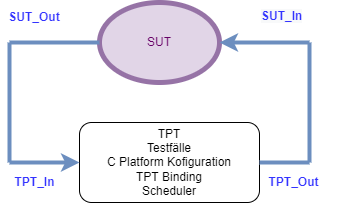
\includegraphics[scale=.6,]{Bilder/Quicktest/SUT_TPT.drawio.png}
\newpage
\section*{\textit{Platform Configuration} und \textit{Platform Execution}}
%zuerst Platform Configuration und Platform Execution und danach C Platform Konfiguration als Überschriften
%Was macht man in der Platform Configuration? Frage beantworten
% Man wählt eine Plattform aus der Plattformkonfiguration aus und 
% In der Plattformkonfiguration 
% Es gibt verschiedene Plattformen, in denen 
Die Plattformkonfigurationen in TPT dienen dazu, das zu testende System in TPT für die Analyse zu konfigurieren.
Eine Plattform ist die C-Platfform, die in dieser Arbeit ausschließlich behandelt wird.
% Es gibt in TPT Plattformen, in denen
% In der Plattformkonfiguration werden 
%Die beiden sind streng getrennt und unabhängig voneinander. Neben der C-Platform Konfiguration gibt es auch noch andere Platformen,
%die aber für diese Arbeit nicht weiter wichtig sind. 
%Es gibt verschiedene Platformkonfigurationen wie beispielsweise die C Platform Konfiguration. 
In der Plattform \textit{Execution} wird festgelegt, welche Tests durchgeführt werden sollen.
Die Plattform Konfiguration und die Plattform \textit{Execution} sind streng getrennt und unabhängig voneinander.
Der große Vorteil dieser Trennung ist, dass die Plattformkonfiguration ausgetauscht werden kann und die Testfälle nicht neu geschrieben
werden müssen. Alle Einstellungen der Plattformkonfiguration sind unabhängig von der Testfallerstellung\parencite[S. 120]{tpt}. 

\section*{C-Plattform Konfiguration}
%es gibt verschiedene voreingestellte Platformen, die man benutzen kann.
Es gibt folgende Konfigurationsmöglichkeiten \parencite[S. 862 ff.]{userguide}:
\begin{description}
\item[Compiler auswählen] Pfad zu einem installierten Compiler
\item[Sourcen auswählen] Diese werden später gelinkt und kompiliert, zu analysierende Sourcen müssen auf analysieren gestellt werden
% dabei werden die ausgewählten Sourcen kompiliert und diejenigen, die auf zu analysieren gestellt sind, werden analysiert
% für GSIL: alle \_Task.c auf set analyze setzen
\item[Scheduler] Ein (Prozess-)Scheduler berechnet und entscheidet, wann und wie lange ein Prozess die CPU Zeit bekommt \parencite[S. 44]{scheduler}.
Hier ist ein Prozess eine Funktion, die ausgeführt wird, sobald sie die CPU Zeit bekommt. %Wenn diese Funktion die CPU Zeit, wird diese ausgeführt. Im 
Im TPT Scheduler werden vom Benutzer Funktionen ausgewählt, die während der Testdurchführung ausgeführt werden sollen.
Es können die ausgewählten Funktionen auf \textit{Startup, Initial} und \textit{Periodic} gestellt werden.
Mit \textit{Startup} wird die Funktion nur einmal am Anfang der Testdurchführung ausgeführt. Mit \textit{Initial} wird die Funktion
einmal am Anfang eines Zyklus ausgeführt und mit \textit{Periodic} wird die Funktion einmal pro definierter Abtastrate ausgeführt.
% Dabei gibt es Startup, wobei die 
% Funktionen, die aufgerufen werden sollen. Hier ist ein Scheduler erklärt \parencite{scheduler}.
\item[Step size] die Abtastrate. Gibt beispielsweise die Zeiteinheit der periodischen Scheduler Funktionen an.
\end{description}
%Test execution und test assessment Oberpunkt weiter nach unten
\section*{\textit{Test Execution} und \textit{Test Assessment}}
Die \textit{Test Execution} und das \textit{Test Assessment} sind zwei getrennte Prozesse.  
Die \textit{Test Execution} ist dafür zuständig die Testfälle auszuführen und dabei Daten zu sammeln. % \parencite[S. 1212 ff.]{userguide}.
Diese gesammelten Daten werden beim \textit{Test Assessment} ausgewertet. 
Daten sind beispielsweise die Werte der Signale, wobei wichtig sein kann, wann und wie lange ein  bestimmter Wert des Signals überschritten wurde \parencite[S. 1212 ff.]{userguide}.
Ein Assessment ist beispielsweise die Auswertung eines Compare Steps.
%, es gibt noch folgende weitere Assessments:
Es gibt auch ein Assessment für Äquivalenzklassen. Dabei kann festgelegt werden, welche Äquivalenzklassen erreicht oder auch nicht erreicht werden sollen \parencite[S. 41 ff.]{tpttutorial}.
%Ein weiteres Assessment ist der Min/Max Vergleich, wobei einzelne Signale detailiert beobachtet werden und festgestellt wird, ob und wie lange ein Signal
%in einem definierten Bereich ist.
% \textit{Test Execution} und \textit{Test Assessment} sind streng getrennt und unabhängig voneinander.
%\parencite[S.41 ff.]{tpttutorial}%Quelle ist nur über Compare Step und Assessment, nicht über Min Max
%Während der \textit{Test Execution} werden Daten aufgesammelt. 
%Daten sind beispielsweise die Werte der Signale im Laufe der Zeit des Tests.
%könnten sein, welche Werte Signale zu welcher Zeit angenommen haben oder welcher Systemzustand gerade aktiv ist.
%Diese Daten werden danach im Assessment ausgewertet. 
% In TPT sind diese beiden streng getrennt. 
% Bei Execution:
% Die Testfälle werden durchgeführt. Die Testfälle sind durch automatons, step lists, Variants definiert.
% Bei der Testdurchführung werden Daten gesammelt.
% Beim Assessment:
% Die gesammelten Daten werden hier ausgewertet. ZB Step list wird ausgewertet.
 % Äquivalenzklasse wird ausgewertet. Die "Check Rules" für die Auswertung werden in 
 % den Assesslets festgelegt.
% In TPT werden Execution und Assessment getrennt und sind unabhängig voneinander

\section*{Analysieren der Dateien}
Durch das Analysieren werden Signale sowie Funktionen der Dateien TPT bekannt gegeben. Es wird auch TPT Binding genannt \parencite[S. 870 ff.]{userguide}.
Das Analysieren erfolgt mit einem Parser. 
Die Aufgabe eines Parsers ist es, Daten auf Korrektheit in Bezug auf einer \glqq Grammatik\grqq{} zu untersuchen und in einer definierten
Struktur intern weiterzuverarbeiten \parencite[S. 1 ff.]{parser}.
%In einem sogenannten TPT Binding werden die Funktionen vom Scheduler sowie die Signale, in TPT Channels genannt, zusammengestellt.
% Channels können auch in TPT importiert werden
% Hier werden Funktionen mit TPT verbunden. Insbesondere können die Channels, die TPT findet,
% übernommen werden oder man importiert die Declarations im Declaration Editor. 

\section*{Generieren und Kompilieren}
Ein Testrahmen wird generiert und inklusive der analysierten Dateien kompiliert.
Neben dem TPT Binding sind auch Scheduling Informationen im Testrahmen zu finden \parencite[S. 868 ff.]{userguide}.
%Mit dem TPT Binding wird ein Testrahmen erstellt und schließlich kompiliert.
% Es wird ein sogenannter Testrahmen erstellt, in dem alle Informationen über das TPT Binding(Channels und Informationen) 
% beinhaltet sind. Schließlich wird es kompiliert.

\section*{Testfallerstellung}
es gibt folgende Steps in der Step Liste \parencite[S. 437 ff.]{userguide}:
\begin{description}
\item[Channel Step] Wertzuweisung auf ein Signal
\item[Compare Step] Ein Signal wird durch das Assessment überprüft, ob es eine definierte Bedingung erfüllt
%\item Channel Step
\item[if, while Step] wie in Programmiersprachen (Java, C++)
\item[wait] Damit läuft die Zeit weiter und Signale können überschrieben werden. Mit @ wird die Zeiteinheit auf die Abtastrate gestellt (siehe C-Plattform Konfiguration Step size).
%läuft die Zeit weiter und eine weitere Sequenz startet, mit @ wird die Wartezeit auf die eingestellte Abtastrate gestellt
% wait Befehl ist nötig, sodass die Zeit weiterlaufen kann und ein weitere Sequenz starten kann.
% Damit wird abgewandt, dass ein Channel einen Kurzschluss hat, indem beispielsweise zwei Werte zur gleichen Zeit
% auf den Channel geschrieben werden.
% wait wie lange?
% am besten mit @
% @ ist eine Referenz auf die eingestellte step size.
\end{description}
Neben der Step Liste gibt es auch noch eine Partition Liste. Diese ermöglicht graphisches Erstellen von Testfallen mithilfe von sogenannten Automatons \parencite[S. 437 ff.]{userguide}.
\section*{\ac{sut}}
In \autoref{fig:SUT_TPT} ist zu sehen, wie das zu testende System mit \ac{tpt} interagiert.
TPT erzeugt im Sinne des Testfalls ein Signal, sendet dieses an das \ac{sut} und
es wird eine Antwort zurück an \ac{tpt} geschickt.
Die Antwort des \ac{sut} wird in \ac{tpt} verarbeitet und gegebenenfalls ein neues Signal an das \ac{sut} geschickt,
wodurch der Zyklus von Neuem beginnt. Es entsteht ein geschlossener Kreis zwischen \ac{sut} und \ac{tpt}.
Dieser Vorgang wird so oft wiederholt, wie es Testfälle gibt \parencite[]{tptsut}.% wodurch ein geschlossener Kreis entsteht.
\begin{figure}[h]
\centering
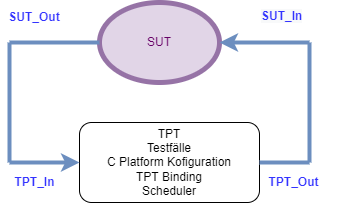
\includegraphics[scale=0.9,]{Bilder/Quicktest/SUT_TPT.drawio.png}
\caption{Zusammenhang zwischen SUT und TPT \parencite{tptsut}}\label{fig:SUT_TPT}
\end{figure}

\section*{TPTAPI}
Mithilfe der TPTAPI kann man das komplette Programm steuern. Die \ac{api} ist in Java geschrieben.
In TPT ist Jython installiert, womit man die Java Module in Python verwenden und TPT steuern kann.
Im Listing C.1 im Anhang sind nützliche Funktionen der TPTAPI aufgezählt \parencite[S. 64 f.]{userguide}.
%Hier werden ein paar nützliche Funktionen vorgestellt:
% \section*{Test Execution und Test Assessment}
% In TPT sind diese beiden streng getrennt. 
% Bei Execution:
% Die Testfälle werden durchgeführt. Die Testfälle sind durch automatons, step lists, Variants definiert.
% Bei der Testdurchführung werden Daten gesammelt.
% Beim Assessment:
% Die gesammelten Daten werden hier ausgewertet. ZB Step list wird ausgewertet.
 % Äquivalenzklasse wird ausgewertet. Die "Check Rules" für die Auswertung werden in 
 % den Assesslets festgelegt.
% In TPT werden Execution und Assessment getrennt und sind unabhängig voneinander

\section*{Äquivalenzklassen}
	% \begin{figure}[h]
% \centering
% 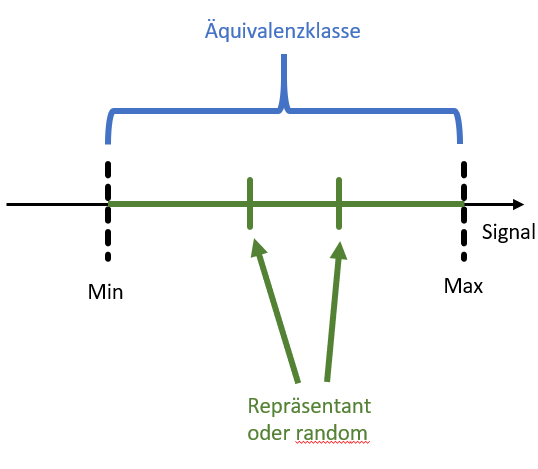
\includegraphics[scale=1.5,]{Bilder/EquiZeitstrahl/ZeitstrahlEineKlasse.png}
% \caption{Äquivalenzklasse in TPT}
% \end{figure}
%\textbf{Darstellung für random, Repräsentanten, Min und Max von Äquivalenzklassen in TPT}
Im \textit{Equivalence Class Set Editor} unter \textit{View} können Äquivalenzklassen definiert werden, um sie 
mehreren Signalen beziehungsweise einem einzigen Signal im Declaration Editor zuzuordnen.
%Die definierten Äquivalenzklassen können im zweiten Schritt Signalen zugeordnet werden.
Sie können als Assesslet \textit{Equivalence Classes} in der Auswertung der Testfälle eingesetzt werden.
%, um zu überprüfen, ob oder ob nicht bestimmte Klassen erreicht werden.
Sie können gleichermaßen in der Step Liste eingesetzt werden, um
Signale auf bestimmte Äquivalenzklassen zu setzen \cite[vgl.][S. 370 ff.]{userguide}.\\
\begin{description}
\item[Assessment]%Ein bild zum Assessment
Mit dem \textit{Equivalence Class Coverage table} können
ausgewählte Testfälle überprüft werden, ob Channels Werte ihrer Äquivalenzklassen
annehmen. In der Report Übersicht wird für jede Äquivalenzklasse der 
gewählten Channels angezeigt, ob und wie oft sie in den gewählten Testfällen vorkommen.
Eine weitere Möglichkeit im Assessment ist, dass 
man forbidden, also verbotene sowie mandatory, verpflichtende
Äquivalenzklassen festlegen kann. Eine Verbotene
besteht den Test, wenn sie nicht eintritt.
Eine Verpflichtende besteht den Test, wenn sie ein
oder mehrere Male eintritt \cite[vgl.][S. 1282 ff.]{userguide}.\\
% Eine verpflichtende Äquivalenzklasse
% kann für ausgewählte 
% Testfälle Channels gesetzt werden. Diese Channels, die Äquivalenzklassen besitzen,
% werden darauf überprüft, ob sie  
% Es wird ein Signal ausgewählt, man kann zwischen mandatory, forbidden und .. auswählen.
% Oben sind 4 Haken zu setzen, diese hier erklären.
\item[Step Liste]%\%ein Bild zur Step Liste
Es gibt vier Schlüsselwörter, um eine Äquivalenzklasse eines Channels
in der Step Liste zu benutzen: \textit{Random, representative, min} und \textit{max}.
Mit \textit{min} und \textit{max} sind jeweils die Grenzen des definierten Wertebereichs gemeint. Mit \textit{random} wird ein zufälliger Wert gewählt, mit \textit{representative} ein Repräsentant.
Wenn kein Schlüsselwort angegeben wird, so wird der Repräsentant gewählt.
Falls kein Repräsentant definiert ist, so wird ein zufälliger Wert innerhalb des Wertebereichs
gewählt \cite[vgl.][S. 379 f.]{userguide}.\\
\item[Äquivalenzklassen von TPT generieren lassen]
Dies kann man mit \textit{Generate Test Cases -> from Equivalence Classes} erreichen.
Man kann auswählen ob sie in einer Step Liste nacheinander
geschrieben werden oder jede in einer 
eigenen Step Liste. Weitere Einstellungsmöglichkeiten sind eine paarweise Kombination und Grenzwerte (siehe Abschnitt 2.2) \cite[vgl.][S. 668 ff.]{userguide}. 
\end{description}
% Generate Test Cases -> from Equivalence Classes 
% Optionen: Auswählen ob Äquivalenzklassen in einzelnen Testfällen, oder alles in einen Testfall als Sequence geschrieben werden

% % Wie erstellt man Äquivalenzklassen in TPT?
% % View -> Equivalence Class Set Editor, Signal in Wertebereich einteilen
% % View -> Declaration Editor Channel(Signal) auf definierte Äquivalenzklasse setzen
% % Assessment -> Equivalence Class auswählen
% % Signale auswählen, mandatory und forbidden equi classes eingeben

% % fertig, jetzt Testdurchführung

% % Äquivalenzklassen von TPT generieren lassen:
% % Generate Test Cases -> from Equivalence Classes 
% % Optionen: Auswählen ob Äquivalenzklassen in einzelnen Testfällen, oder alles in einen Testfall als Sequence geschrieben werden

% % Möglichkeiten der Test Case Erstellung mit Äquivalenzklassen
% % mit Signal.ec->high etc., Repräsentanten und andere Funktionen

% % Dieses Kapitel zu TPT Analyse